% Options for packages loaded elsewhere
\PassOptionsToPackage{unicode}{hyperref}
\PassOptionsToPackage{hyphens}{url}
%
\documentclass[
]{article}
\usepackage{lmodern}
\usepackage{amssymb,amsmath}
\usepackage{ifxetex,ifluatex}
\ifnum 0\ifxetex 1\fi\ifluatex 1\fi=0 % if pdftex
  \usepackage[T1]{fontenc}
  \usepackage[utf8]{inputenc}
  \usepackage{textcomp} % provide euro and other symbols
\else % if luatex or xetex
  \usepackage{unicode-math}
  \defaultfontfeatures{Scale=MatchLowercase}
  \defaultfontfeatures[\rmfamily]{Ligatures=TeX,Scale=1}
\fi
% Use upquote if available, for straight quotes in verbatim environments
\IfFileExists{upquote.sty}{\usepackage{upquote}}{}
\IfFileExists{microtype.sty}{% use microtype if available
  \usepackage[]{microtype}
  \UseMicrotypeSet[protrusion]{basicmath} % disable protrusion for tt fonts
}{}
\makeatletter
\@ifundefined{KOMAClassName}{% if non-KOMA class
  \IfFileExists{parskip.sty}{%
    \usepackage{parskip}
  }{% else
    \setlength{\parindent}{0pt}
    \setlength{\parskip}{6pt plus 2pt minus 1pt}}
}{% if KOMA class
  \KOMAoptions{parskip=half}}
\makeatother
\usepackage{xcolor}
\IfFileExists{xurl.sty}{\usepackage{xurl}}{} % add URL line breaks if available
\IfFileExists{bookmark.sty}{\usepackage{bookmark}}{\usepackage{hyperref}}
\hypersetup{
  pdftitle={FIT3152asm\_1\_final\_markdown},
  hidelinks,
  pdfcreator={LaTeX via pandoc}}
\urlstyle{same} % disable monospaced font for URLs
\usepackage[margin=1in]{geometry}
\usepackage{color}
\usepackage{fancyvrb}
\newcommand{\VerbBar}{|}
\newcommand{\VERB}{\Verb[commandchars=\\\{\}]}
\DefineVerbatimEnvironment{Highlighting}{Verbatim}{commandchars=\\\{\}}
% Add ',fontsize=\small' for more characters per line
\usepackage{framed}
\definecolor{shadecolor}{RGB}{248,248,248}
\newenvironment{Shaded}{\begin{snugshade}}{\end{snugshade}}
\newcommand{\AlertTok}[1]{\textcolor[rgb]{0.94,0.16,0.16}{#1}}
\newcommand{\AnnotationTok}[1]{\textcolor[rgb]{0.56,0.35,0.01}{\textbf{\textit{#1}}}}
\newcommand{\AttributeTok}[1]{\textcolor[rgb]{0.77,0.63,0.00}{#1}}
\newcommand{\BaseNTok}[1]{\textcolor[rgb]{0.00,0.00,0.81}{#1}}
\newcommand{\BuiltInTok}[1]{#1}
\newcommand{\CharTok}[1]{\textcolor[rgb]{0.31,0.60,0.02}{#1}}
\newcommand{\CommentTok}[1]{\textcolor[rgb]{0.56,0.35,0.01}{\textit{#1}}}
\newcommand{\CommentVarTok}[1]{\textcolor[rgb]{0.56,0.35,0.01}{\textbf{\textit{#1}}}}
\newcommand{\ConstantTok}[1]{\textcolor[rgb]{0.00,0.00,0.00}{#1}}
\newcommand{\ControlFlowTok}[1]{\textcolor[rgb]{0.13,0.29,0.53}{\textbf{#1}}}
\newcommand{\DataTypeTok}[1]{\textcolor[rgb]{0.13,0.29,0.53}{#1}}
\newcommand{\DecValTok}[1]{\textcolor[rgb]{0.00,0.00,0.81}{#1}}
\newcommand{\DocumentationTok}[1]{\textcolor[rgb]{0.56,0.35,0.01}{\textbf{\textit{#1}}}}
\newcommand{\ErrorTok}[1]{\textcolor[rgb]{0.64,0.00,0.00}{\textbf{#1}}}
\newcommand{\ExtensionTok}[1]{#1}
\newcommand{\FloatTok}[1]{\textcolor[rgb]{0.00,0.00,0.81}{#1}}
\newcommand{\FunctionTok}[1]{\textcolor[rgb]{0.00,0.00,0.00}{#1}}
\newcommand{\ImportTok}[1]{#1}
\newcommand{\InformationTok}[1]{\textcolor[rgb]{0.56,0.35,0.01}{\textbf{\textit{#1}}}}
\newcommand{\KeywordTok}[1]{\textcolor[rgb]{0.13,0.29,0.53}{\textbf{#1}}}
\newcommand{\NormalTok}[1]{#1}
\newcommand{\OperatorTok}[1]{\textcolor[rgb]{0.81,0.36,0.00}{\textbf{#1}}}
\newcommand{\OtherTok}[1]{\textcolor[rgb]{0.56,0.35,0.01}{#1}}
\newcommand{\PreprocessorTok}[1]{\textcolor[rgb]{0.56,0.35,0.01}{\textit{#1}}}
\newcommand{\RegionMarkerTok}[1]{#1}
\newcommand{\SpecialCharTok}[1]{\textcolor[rgb]{0.00,0.00,0.00}{#1}}
\newcommand{\SpecialStringTok}[1]{\textcolor[rgb]{0.31,0.60,0.02}{#1}}
\newcommand{\StringTok}[1]{\textcolor[rgb]{0.31,0.60,0.02}{#1}}
\newcommand{\VariableTok}[1]{\textcolor[rgb]{0.00,0.00,0.00}{#1}}
\newcommand{\VerbatimStringTok}[1]{\textcolor[rgb]{0.31,0.60,0.02}{#1}}
\newcommand{\WarningTok}[1]{\textcolor[rgb]{0.56,0.35,0.01}{\textbf{\textit{#1}}}}
\usepackage{graphicx,grffile}
\makeatletter
\def\maxwidth{\ifdim\Gin@nat@width>\linewidth\linewidth\else\Gin@nat@width\fi}
\def\maxheight{\ifdim\Gin@nat@height>\textheight\textheight\else\Gin@nat@height\fi}
\makeatother
% Scale images if necessary, so that they will not overflow the page
% margins by default, and it is still possible to overwrite the defaults
% using explicit options in \includegraphics[width, height, ...]{}
\setkeys{Gin}{width=\maxwidth,height=\maxheight,keepaspectratio}
% Set default figure placement to htbp
\makeatletter
\def\fps@figure{htbp}
\makeatother
\setlength{\emergencystretch}{3em} % prevent overfull lines
\providecommand{\tightlist}{%
  \setlength{\itemsep}{0pt}\setlength{\parskip}{0pt}}
\setcounter{secnumdepth}{-\maxdimen} % remove section numbering

\title{FIT3152asm\_1\_final\_markdown}
\author{}
\date{\vspace{-2.5em}}

\begin{document}
\maketitle

Import needed library

\begin{Shaded}
\begin{Highlighting}[]
\KeywordTok{library}\NormalTok{(tidyverse)}
\KeywordTok{library}\NormalTok{(lubridate)}
\end{Highlighting}
\end{Shaded}

Read the data

\begin{Shaded}
\begin{Highlighting}[]
\KeywordTok{rm}\NormalTok{(}\DataTypeTok{list =} \KeywordTok{ls}\NormalTok{())}
\KeywordTok{set.seed}\NormalTok{(}\DecValTok{31084222}\NormalTok{)}
\NormalTok{data <-}\StringTok{  }\KeywordTok{read.csv}\NormalTok{(}\StringTok{"C:/Users/sjsa3/Desktop/Shared_with_Mac/year2_sem1/FIT3152/Assignment_FIT3152_2021/webforum.csv"}\NormalTok{)}

\NormalTok{data <-}\StringTok{ }\NormalTok{data[}\KeywordTok{sample}\NormalTok{(}\KeywordTok{nrow}\NormalTok{(data),}\DecValTok{20000}\NormalTok{),] }\CommentTok{#20000 rows}
\end{Highlighting}
\end{Shaded}

Clean the data

\begin{Shaded}
\begin{Highlighting}[]
\CommentTok{#define Min-Max normalisation method}
\NormalTok{min_max_normalisation <-}\StringTok{ }\ControlFlowTok{function}\NormalTok{(x) \{}
\NormalTok{    (x }\OperatorTok{-}\StringTok{ }\KeywordTok{min}\NormalTok{(x)) }\OperatorTok{/}\StringTok{ }\NormalTok{(}\KeywordTok{max}\NormalTok{(x) }\OperatorTok{-}\StringTok{ }\KeywordTok{min}\NormalTok{(x))}
\NormalTok{  \}}
\end{Highlighting}
\end{Shaded}

\begin{Shaded}
\begin{Highlighting}[]
\NormalTok{data}\OperatorTok{$}\NormalTok{Date <-}\StringTok{ }\KeywordTok{as.Date}\NormalTok{(data}\OperatorTok{$}\NormalTok{Date)}


\CommentTok{#check if there is any missing values}
\KeywordTok{sum}\NormalTok{(}\KeywordTok{is.na}\NormalTok{(data))}
\end{Highlighting}
\end{Shaded}

\begin{verbatim}
## [1] 0
\end{verbatim}

\begin{Shaded}
\begin{Highlighting}[]
\NormalTok{data_tidy <-}\StringTok{ }\NormalTok{data }\OperatorTok
\StringTok{  }\KeywordTok{mutate}\NormalTok{(}\DataTypeTok{month =} \KeywordTok{month}\NormalTok{(Date,  }\DataTypeTok{label =} \OtherTok{TRUE}\NormalTok{, }\DataTypeTok{abbr =} \OtherTok{TRUE}\NormalTok{), }
         \DataTypeTok{wday =} \KeywordTok{wday}\NormalTok{(Date, }\DataTypeTok{label =} \OtherTok{TRUE}\NormalTok{, }\DataTypeTok{abbr =} \OtherTok{TRUE}\NormalTok{, }\DataTypeTok{week_start =} \DecValTok{1}\NormalTok{),}
         \DataTypeTok{year =} \KeywordTok{year}\NormalTok{(Date),}
         \DataTypeTok{day =} \KeywordTok{day}\NormalTok{(Date),}
         \DataTypeTok{hour =}  \KeywordTok{hour}\NormalTok{(}\KeywordTok{hm}\NormalTok{(data}\OperatorTok{$}\NormalTok{Time)))}

  
\CommentTok{#apply Min-Max normalisation to all numeric columns}
\NormalTok{data_tidy_norm <-}\StringTok{ }\KeywordTok{as.data.frame}\NormalTok{(}\KeywordTok{lapply}\NormalTok{(data_tidy[,}\DecValTok{5}\OperatorTok{:}\DecValTok{19}\NormalTok{], min_max_normalisation))}

\CommentTok{#scale the data}
\NormalTok{data_tidy_scale <-}\StringTok{ }\KeywordTok{as.data.frame}\NormalTok{(}\KeywordTok{scale}\NormalTok{(data_tidy[}\DecValTok{5}\OperatorTok{:}\DecValTok{19}\NormalTok{]))}
\end{Highlighting}
\end{Shaded}

==============================================================================================================
- Q2

\begin{verbatim}
Analyse the language used by groups. Some starting points:



b By analysing the linguistic variables for all or some of the threads, is it possible to see a
difference in the language used by different groups?
--------------------------------------------------------------------------------------------

1. find out the 10 most active threads
\end{verbatim}

\begin{Shaded}
\begin{Highlighting}[]
\NormalTok{data_tidy_norm <-}\StringTok{ }\NormalTok{data_tidy_norm }\OperatorTok\StringTok{ }\KeywordTok{cbind}\NormalTok{(}\DataTypeTok{ThreadID =}\NormalTok{ data_tidy}\OperatorTok{$}\NormalTok{ThreadID)}
\NormalTok{df_active_}\DecValTok{10}\NormalTok{ <-}\StringTok{  }\NormalTok{data_tidy }\OperatorTok\StringTok{ }\KeywordTok{group_by}\NormalTok{(ThreadID)}\OperatorTok\StringTok{ }\KeywordTok{summarise}\NormalTok{(}\DataTypeTok{count =} \KeywordTok{n}\NormalTok{()) }\OperatorTok\StringTok{ }\KeywordTok{arrange}\NormalTok{(}\KeywordTok{desc}\NormalTok{(count))}
\end{Highlighting}
\end{Shaded}

\begin{verbatim}
## `summarise()` ungrouping output (override with `.groups` argument)
\end{verbatim}

\begin{Shaded}
\begin{Highlighting}[]
\NormalTok{df_active_}\DecValTok{10}\NormalTok{ <-}\StringTok{ }\KeywordTok{head}\NormalTok{(df_active_}\DecValTok{10}\NormalTok{,}\DecValTok{10}\NormalTok{)}
\NormalTok{df_active_}\DecValTok{10}
\end{Highlighting}
\end{Shaded}

\begin{verbatim}
## # A tibble: 10 x 2
##    ThreadID count
##       <int> <int>
##  1   283958   136
##  2   252620   127
##  3   127115   114
##  4   472752   109
##  5   145223    95
##  6   532649    79
##  7   309286    71
##  8   191868    69
##  9   296985    65
## 10   249001    56
\end{verbatim}

\begin{Shaded}
\begin{Highlighting}[]
\NormalTok{df <-}\StringTok{  }\NormalTok{data_tidy }\OperatorTok\StringTok{ }\KeywordTok{filter}\NormalTok{(data_tidy_norm}\OperatorTok{$}\NormalTok{ThreadID }\OperatorTok\StringTok{ }\NormalTok{df_active_}\DecValTok{10}\OperatorTok{$}\NormalTok{ThreadID  ) }\OperatorTok\StringTok{ }\KeywordTok{arrange}\NormalTok{(ThreadID)}
\end{Highlighting}
\end{Shaded}

\begin{Shaded}
\begin{Highlighting}[]
\KeywordTok{library}\NormalTok{(}\StringTok{"corrgram"}\NormalTok{)}
\end{Highlighting}
\end{Shaded}

\begin{verbatim}
## Warning: package 'corrgram' was built under R version 4.0.4
\end{verbatim}

\begin{Shaded}
\begin{Highlighting}[]
\KeywordTok{corrgram}\NormalTok{(df,}\DataTypeTok{upper.panel=}\NormalTok{panel.cor)}
\end{Highlighting}
\end{Shaded}

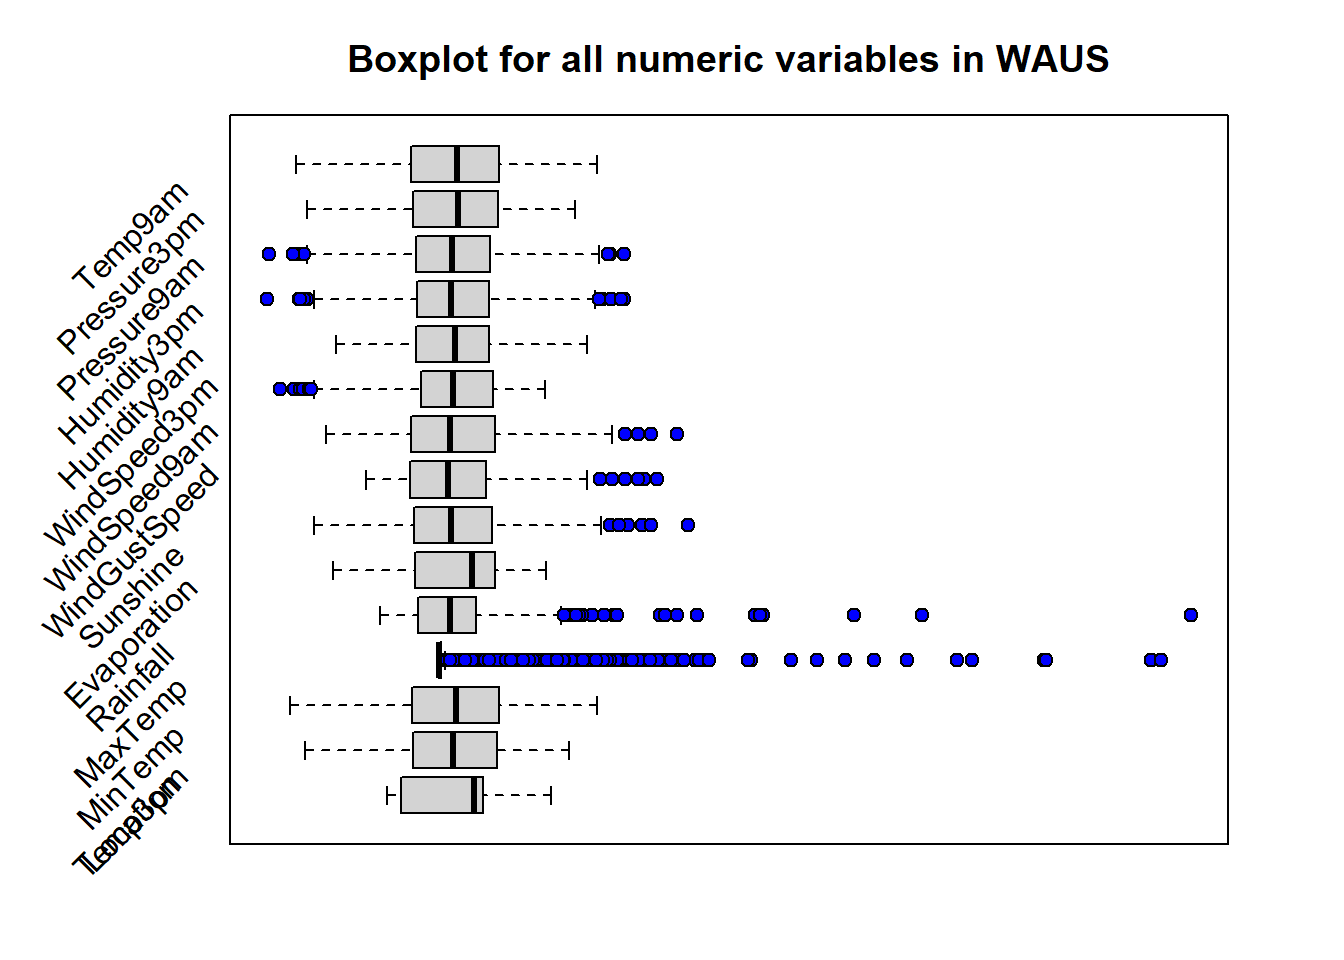
\includegraphics{Q2_files/figure-latex/unnamed-chunk-2-1.pdf}

\begin{verbatim}
Relationship :
2. corrogram 
3. see if there is any relationship

Tone : 
4. Which one is the most positvie
\end{verbatim}

\begin{Shaded}
\begin{Highlighting}[]
\NormalTok{data_nega_pose =}\StringTok{ }\NormalTok{df }\OperatorTok\StringTok{ }\KeywordTok{group_by}\NormalTok{(ThreadID) }\OperatorTok\StringTok{ }\KeywordTok{summarise}\NormalTok{(}\DataTypeTok{mean =} \KeywordTok{mean}\NormalTok{(Tone))}
\end{Highlighting}
\end{Shaded}

\begin{verbatim}
## `summarise()` ungrouping output (override with `.groups` argument)
\end{verbatim}

\begin{Shaded}
\begin{Highlighting}[]
\NormalTok{data_nega_pose =}\StringTok{ }\NormalTok{data_nega_pose }\OperatorTok\StringTok{ }\KeywordTok{mutate}\NormalTok{(}\DataTypeTok{emo =} \KeywordTok{ifelse}\NormalTok{(mean }\OperatorTok{>}\DecValTok{50}\NormalTok{ , }\StringTok{"Positive"}\NormalTok{, }\StringTok{"Negative"}\NormalTok{))}\OperatorTok\StringTok{ }
\StringTok{  }\KeywordTok{group_by}\NormalTok{(emo) }\OperatorTok\StringTok{ }\KeywordTok{arrange}\NormalTok{(}\KeywordTok{desc}\NormalTok{(mean))}
\end{Highlighting}
\end{Shaded}

\begin{verbatim}
What languages used to shape this Tone?
1.Pick the most postive and negative one to analyse 
\end{verbatim}

\begin{Shaded}
\begin{Highlighting}[]
\CommentTok{#most positve}
\NormalTok{data.mostPose <-}\StringTok{ }\NormalTok{data_tidy }\OperatorTok\StringTok{ }\KeywordTok{filter}\NormalTok{(ThreadID }\OperatorTok{==}\StringTok{"472752"}\NormalTok{ )}
\NormalTok{data.mostPose <-}\StringTok{ }\NormalTok{data.mostPose[}\DecValTok{5}\OperatorTok{:}\DecValTok{19}\NormalTok{]}
\CommentTok{# corrgram(data.mostPose,upper.panel=panel.cor)}

\CommentTok{#most negative}
\NormalTok{data.mostNega <-}\StringTok{ }\NormalTok{data_tidy }\OperatorTok\StringTok{ }\KeywordTok{filter}\NormalTok{(ThreadID }\OperatorTok{==}\StringTok{"309286"}\NormalTok{ )}
\NormalTok{data.mostNega <-}\StringTok{ }\NormalTok{data.mostNega[}\DecValTok{5}\OperatorTok{:}\DecValTok{19}\NormalTok{]}
\CommentTok{# corrgram(data.mostNega,upper.panel=panel.cor)}

\NormalTok{data_emo <-}\StringTok{ }\NormalTok{data_tidy_norm }\OperatorTok\StringTok{ }\KeywordTok{filter}\NormalTok{(ThreadID }\OperatorTok\StringTok{ }\KeywordTok{c}\NormalTok{(}\StringTok{"309286"}\NormalTok{, }\StringTok{"472752"}\NormalTok{)  ) }\OperatorTok
\StringTok{  }\KeywordTok{group_by}\NormalTok{(ThreadID)}\OperatorTok\StringTok{  }
\StringTok{  }\KeywordTok{summarise}\NormalTok{(}\DataTypeTok{WPS_mean=}\KeywordTok{mean}\NormalTok{(WPS), }\DataTypeTok{WC_mean =} \KeywordTok{mean}\NormalTok{(WC),}
            \DataTypeTok{i_mean =} \KeywordTok{mean}\NormalTok{(i),}
            \DataTypeTok{we_mean =} \KeywordTok{mean}\NormalTok{(we),}
            \DataTypeTok{you_mean =} \KeywordTok{mean}\NormalTok{(you),}
            \DataTypeTok{they_mean =} \KeywordTok{mean}\NormalTok{(they ),}
            \DataTypeTok{Clout_mean=} \KeywordTok{mean}\NormalTok{(Clout))}
\end{Highlighting}
\end{Shaded}

\begin{verbatim}
## `summarise()` ungrouping output (override with `.groups` argument)
\end{verbatim}

\begin{Shaded}
\begin{Highlighting}[]
\KeywordTok{library}\NormalTok{(fmsb)}
\NormalTok{data.mostPose <-}\StringTok{ }\NormalTok{data.mostPose }\OperatorTok\StringTok{ }\KeywordTok{select}\NormalTok{(Analytic,Clout,Authentic,WC,WPS,affect)}\OperatorTok\StringTok{ }
\StringTok{  }\KeywordTok{mutate}\NormalTok{(}\DataTypeTok{Pronoun =}\NormalTok{ data.mostPose[,}\DecValTok{7}\NormalTok{] }\OperatorTok{+}\StringTok{ }\NormalTok{data.mostPose[,}\DecValTok{8}\NormalTok{]}\OperatorTok{+}\StringTok{ }\NormalTok{data.mostPose[,}\DecValTok{9}\NormalTok{] }\OperatorTok{+}\StringTok{  }\NormalTok{data.mostPose[,}\DecValTok{10}\NormalTok{] )}


\NormalTok{data.mostPose <-}\StringTok{ }\KeywordTok{as.data.frame}\NormalTok{(}\KeywordTok{lapply}\NormalTok{(data.mostPose[,], min_max_normalisation))}
\NormalTok{data.mostPose <-}\StringTok{ }\NormalTok{data.mostPose }\OperatorTok\StringTok{ }\KeywordTok{summarise}\NormalTok{(}\DataTypeTok{Analytic_m =} \KeywordTok{mean}\NormalTok{(Analytic)}\OperatorTok{*}\DecValTok{100}\NormalTok{,}
                                             \DataTypeTok{Clout_m =} \KeywordTok{mean}\NormalTok{(Clout)}\OperatorTok{*}\DecValTok{100}\NormalTok{,}
                                             \DataTypeTok{Authentic_m =} \KeywordTok{mean}\NormalTok{(Authentic)}\OperatorTok{*}\DecValTok{100}\NormalTok{,}
                                            \DataTypeTok{WC_m =} \KeywordTok{mean}\NormalTok{(WC)}\OperatorTok{*}\DecValTok{100}\NormalTok{,}
                                            \DataTypeTok{WPS_m =} \KeywordTok{mean}\NormalTok{(WPS)}\OperatorTok{*}\DecValTok{100}\NormalTok{,}
                                            \DataTypeTok{affect_m =} \KeywordTok{mean}\NormalTok{(affect)}\OperatorTok{*}\DecValTok{100}\NormalTok{,}
                                             \DataTypeTok{Pronoun_m =} \KeywordTok{mean}\NormalTok{(Pronoun)}\OperatorTok{*}\DecValTok{100}\NormalTok{,}
\NormalTok{                                             )}

\CommentTok{# negative}
\NormalTok{data.mostNega <-}\StringTok{ }\NormalTok{data.mostNega }\OperatorTok\StringTok{ }\KeywordTok{select}\NormalTok{(Analytic,Clout,Authentic,WC,WPS,affect)}\OperatorTok\StringTok{ }
\StringTok{  }\KeywordTok{mutate}\NormalTok{(}\DataTypeTok{Pronoun =}\NormalTok{ data.mostNega[,}\DecValTok{7}\NormalTok{] }\OperatorTok{+}\StringTok{ }\NormalTok{data.mostNega[,}\DecValTok{8}\NormalTok{]}\OperatorTok{+}\StringTok{ }\NormalTok{data.mostNega[,}\DecValTok{9}\NormalTok{] }\OperatorTok{+}\StringTok{  }\NormalTok{data.mostNega[,}\DecValTok{10}\NormalTok{] )}


\NormalTok{data.mostNega <-}\StringTok{ }\KeywordTok{as.data.frame}\NormalTok{(}\KeywordTok{lapply}\NormalTok{(data.mostNega[,], min_max_normalisation))}
\NormalTok{data.mostNega <-}\StringTok{ }\NormalTok{data.mostNega }\OperatorTok\StringTok{ }\KeywordTok{summarise}\NormalTok{(}\DataTypeTok{Analytic_m =} \KeywordTok{mean}\NormalTok{(Analytic)}\OperatorTok{*}\DecValTok{100}\NormalTok{,}
                                             \DataTypeTok{Clout_m =} \KeywordTok{mean}\NormalTok{(Clout)}\OperatorTok{*}\DecValTok{100}\NormalTok{,}
                                             \DataTypeTok{Authentic_m =} \KeywordTok{mean}\NormalTok{(Authentic)}\OperatorTok{*}\DecValTok{100}\NormalTok{,}
                                            \DataTypeTok{WC_m =} \KeywordTok{mean}\NormalTok{(WC)}\OperatorTok{*}\DecValTok{100}\NormalTok{,}
                                            \DataTypeTok{WPS_m =} \KeywordTok{mean}\NormalTok{(WPS)}\OperatorTok{*}\DecValTok{100}\NormalTok{,}
                                            \DataTypeTok{affect_m =} \KeywordTok{mean}\NormalTok{(affect)}\OperatorTok{*}\DecValTok{100}\NormalTok{,}
                                             \DataTypeTok{Pronoun_m =} \KeywordTok{mean}\NormalTok{(Pronoun)}\OperatorTok{*}\DecValTok{100}\NormalTok{,}
\NormalTok{                                             )}

\NormalTok{radar_data_Pose <-}\StringTok{ }\NormalTok{data.mostNega }\OperatorTok\StringTok{ }\KeywordTok{rbind}\NormalTok{(data.mostPose )}



\NormalTok{radar_data_Pose <-}\KeywordTok{data.frame}\NormalTok{( }\DataTypeTok{Analytic =} \KeywordTok{c}\NormalTok{(}\DecValTok{100}\NormalTok{, }\DecValTok{0}\NormalTok{ , data.mostPose[}\DecValTok{1}\NormalTok{,}\DecValTok{1}\NormalTok{],data.mostNega[}\DecValTok{1}\NormalTok{,}\DecValTok{1}\NormalTok{] ),}
                              \DataTypeTok{Clout =} \KeywordTok{c}\NormalTok{(}\DecValTok{100}\NormalTok{, }\DecValTok{0}\NormalTok{ , data.mostPose[}\DecValTok{1}\NormalTok{,}\DecValTok{2}\NormalTok{],data.mostNega[}\DecValTok{1}\NormalTok{,}\DecValTok{2}\NormalTok{]  ),}
                              \DataTypeTok{Authentic =} \KeywordTok{c}\NormalTok{(}\DecValTok{100}\NormalTok{, }\DecValTok{0}\NormalTok{ , data.mostPose[}\DecValTok{1}\NormalTok{,}\DecValTok{3}\NormalTok{],data.mostNega[}\DecValTok{1}\NormalTok{,}\DecValTok{3}\NormalTok{]  ),}
                              \DataTypeTok{WC =} \KeywordTok{c}\NormalTok{(}\DecValTok{100}\NormalTok{, }\DecValTok{0}\NormalTok{ , data.mostPose[}\DecValTok{1}\NormalTok{,}\DecValTok{4}\NormalTok{],data.mostNega[}\DecValTok{1}\NormalTok{,}\DecValTok{4}\NormalTok{]  ),}
                              \DataTypeTok{WPS =} \KeywordTok{c}\NormalTok{(}\DecValTok{100}\NormalTok{, }\DecValTok{0}\NormalTok{ , data.mostPose[}\DecValTok{1}\NormalTok{,}\DecValTok{5}\NormalTok{],data.mostNega[}\DecValTok{1}\NormalTok{,}\DecValTok{5}\NormalTok{]  ),}
                              \DataTypeTok{affect =} \KeywordTok{c}\NormalTok{(}\DecValTok{100}\NormalTok{, }\DecValTok{0}\NormalTok{ , data.mostPose[}\DecValTok{1}\NormalTok{,}\DecValTok{6}\NormalTok{],data.mostNega[}\DecValTok{1}\NormalTok{,}\DecValTok{6}\NormalTok{]  ),}
                              \DataTypeTok{Pronoun =} \KeywordTok{c}\NormalTok{(}\DecValTok{100}\NormalTok{, }\DecValTok{0}\NormalTok{ , data.mostPose[}\DecValTok{1}\NormalTok{,}\DecValTok{7}\NormalTok{],data.mostNega[}\DecValTok{1}\NormalTok{,}\DecValTok{7}\NormalTok{]  ),}
                              \DataTypeTok{row.names =} \KeywordTok{c}\NormalTok{(}\StringTok{"max"}\NormalTok{,}\StringTok{"min"}\NormalTok{,}\StringTok{"P"}\NormalTok{,}\StringTok{"N"}\NormalTok{)}
\NormalTok{                              )}
\CommentTok{#defien the colors filled}
\NormalTok{colors_fill <-}\StringTok{ }\KeywordTok{c}\NormalTok{(scales}\OperatorTok{::}\KeywordTok{alpha}\NormalTok{(}\StringTok{"blue"}\NormalTok{, }\FloatTok{0.3}\NormalTok{),scales}\OperatorTok{::}\KeywordTok{alpha}\NormalTok{(}\StringTok{"red"}\NormalTok{, }\FloatTok{0.5}\NormalTok{))}
\CommentTok{#define the line colors}
\NormalTok{colors_line <-}\StringTok{ }\KeywordTok{c}\NormalTok{(scales}\OperatorTok{::}\KeywordTok{alpha}\NormalTok{(}\StringTok{"black"}\NormalTok{, }\FloatTok{0.5}\NormalTok{),scales}\OperatorTok{::}\KeywordTok{alpha}\NormalTok{(}\StringTok{"darkgrey"}\NormalTok{, }\FloatTok{0.5}\NormalTok{))}
\KeywordTok{radarchart}\NormalTok{(radar_data_Pose, }\DataTypeTok{axistype =} \DecValTok{1}\NormalTok{,}
           \DataTypeTok{seg =} \DecValTok{2}\NormalTok{,}
    \CommentTok{# Customize the polygon}
     \DataTypeTok{pfcol =}\NormalTok{colors_fill, }\DataTypeTok{plwd =} \DecValTok{2}\NormalTok{, }\DataTypeTok{plty =} \DecValTok{1}\NormalTok{,}
    \CommentTok{# Customize the grid}
    \DataTypeTok{cglcol =} \StringTok{"grey"}\NormalTok{, }\DataTypeTok{cglty =} \DecValTok{1}\NormalTok{, }\DataTypeTok{cglwd =} \FloatTok{0.8}\NormalTok{,}
    \DataTypeTok{pcol =}\NormalTok{ colors_line,}
    \CommentTok{# Customize the axis}
    \DataTypeTok{axislabcol =} \StringTok{"grey"}\NormalTok{,}
    \DataTypeTok{caxislabels =} \KeywordTok{c}\NormalTok{(}\DecValTok{0}\NormalTok{, }\DecValTok{50}\NormalTok{, }\DecValTok{100}\NormalTok{))}
           
\KeywordTok{legend}\NormalTok{( }\DataTypeTok{x=}\FloatTok{0.6}\NormalTok{,}\DataTypeTok{y=}\FloatTok{1.35}\NormalTok{,}\DataTypeTok{legend =} \KeywordTok{row.names}\NormalTok{( radar_data_Pose[}\DecValTok{3}\OperatorTok{:}\DecValTok{4}\NormalTok{,] ) ,}
        \DataTypeTok{bty =} \StringTok{"n"}\NormalTok{,}
        \DataTypeTok{pch =} \DecValTok{20}\NormalTok{,}
        \DataTypeTok{col=}\NormalTok{colors_fill,}
        \DataTypeTok{cex=}\FloatTok{1.2}\NormalTok{,}
        \DataTypeTok{pt.cex=}\DecValTok{3}\NormalTok{)}
\end{Highlighting}
\end{Shaded}

\includegraphics{Q2_files/figure-latex/radar-chart-all-1.pdf}

\begin{verbatim}
c Does the language used within threads (or between threads) change over time? How
    consistent or variable is the language used within threads?
--------------------------------------------------------------------------------------------
    
    
    
    
    
    
    
    
    
    
    
    
\end{verbatim}

\end{document}
